% Options for packages loaded elsewhere
\PassOptionsToPackage{unicode}{hyperref}
\PassOptionsToPackage{hyphens}{url}
%
\documentclass[
]{book}
\usepackage{amsmath,amssymb}
\usepackage{lmodern}
\usepackage{iftex}
\ifPDFTeX
  \usepackage[T1]{fontenc}
  \usepackage[utf8]{inputenc}
  \usepackage{textcomp} % provide euro and other symbols
\else % if luatex or xetex
  \usepackage{unicode-math}
  \defaultfontfeatures{Scale=MatchLowercase}
  \defaultfontfeatures[\rmfamily]{Ligatures=TeX,Scale=1}
\fi
% Use upquote if available, for straight quotes in verbatim environments
\IfFileExists{upquote.sty}{\usepackage{upquote}}{}
\IfFileExists{microtype.sty}{% use microtype if available
  \usepackage[]{microtype}
  \UseMicrotypeSet[protrusion]{basicmath} % disable protrusion for tt fonts
}{}
\makeatletter
\@ifundefined{KOMAClassName}{% if non-KOMA class
  \IfFileExists{parskip.sty}{%
    \usepackage{parskip}
  }{% else
    \setlength{\parindent}{0pt}
    \setlength{\parskip}{6pt plus 2pt minus 1pt}}
}{% if KOMA class
  \KOMAoptions{parskip=half}}
\makeatother
\usepackage{xcolor}
\IfFileExists{xurl.sty}{\usepackage{xurl}}{} % add URL line breaks if available
\IfFileExists{bookmark.sty}{\usepackage{bookmark}}{\usepackage{hyperref}}
\hypersetup{
  pdftitle={INTRODUCCIÓN A LA ESTABILIDAD FINANCIERA},
  pdfauthor={LUIS ORTIZ-CEVALLOS},
  hidelinks,
  pdfcreator={LaTeX via pandoc}}
\urlstyle{same} % disable monospaced font for URLs
\usepackage{color}
\usepackage{fancyvrb}
\newcommand{\VerbBar}{|}
\newcommand{\VERB}{\Verb[commandchars=\\\{\}]}
\DefineVerbatimEnvironment{Highlighting}{Verbatim}{commandchars=\\\{\}}
% Add ',fontsize=\small' for more characters per line
\usepackage{framed}
\definecolor{shadecolor}{RGB}{248,248,248}
\newenvironment{Shaded}{\begin{snugshade}}{\end{snugshade}}
\newcommand{\AlertTok}[1]{\textcolor[rgb]{0.94,0.16,0.16}{#1}}
\newcommand{\AnnotationTok}[1]{\textcolor[rgb]{0.56,0.35,0.01}{\textbf{\textit{#1}}}}
\newcommand{\AttributeTok}[1]{\textcolor[rgb]{0.77,0.63,0.00}{#1}}
\newcommand{\BaseNTok}[1]{\textcolor[rgb]{0.00,0.00,0.81}{#1}}
\newcommand{\BuiltInTok}[1]{#1}
\newcommand{\CharTok}[1]{\textcolor[rgb]{0.31,0.60,0.02}{#1}}
\newcommand{\CommentTok}[1]{\textcolor[rgb]{0.56,0.35,0.01}{\textit{#1}}}
\newcommand{\CommentVarTok}[1]{\textcolor[rgb]{0.56,0.35,0.01}{\textbf{\textit{#1}}}}
\newcommand{\ConstantTok}[1]{\textcolor[rgb]{0.00,0.00,0.00}{#1}}
\newcommand{\ControlFlowTok}[1]{\textcolor[rgb]{0.13,0.29,0.53}{\textbf{#1}}}
\newcommand{\DataTypeTok}[1]{\textcolor[rgb]{0.13,0.29,0.53}{#1}}
\newcommand{\DecValTok}[1]{\textcolor[rgb]{0.00,0.00,0.81}{#1}}
\newcommand{\DocumentationTok}[1]{\textcolor[rgb]{0.56,0.35,0.01}{\textbf{\textit{#1}}}}
\newcommand{\ErrorTok}[1]{\textcolor[rgb]{0.64,0.00,0.00}{\textbf{#1}}}
\newcommand{\ExtensionTok}[1]{#1}
\newcommand{\FloatTok}[1]{\textcolor[rgb]{0.00,0.00,0.81}{#1}}
\newcommand{\FunctionTok}[1]{\textcolor[rgb]{0.00,0.00,0.00}{#1}}
\newcommand{\ImportTok}[1]{#1}
\newcommand{\InformationTok}[1]{\textcolor[rgb]{0.56,0.35,0.01}{\textbf{\textit{#1}}}}
\newcommand{\KeywordTok}[1]{\textcolor[rgb]{0.13,0.29,0.53}{\textbf{#1}}}
\newcommand{\NormalTok}[1]{#1}
\newcommand{\OperatorTok}[1]{\textcolor[rgb]{0.81,0.36,0.00}{\textbf{#1}}}
\newcommand{\OtherTok}[1]{\textcolor[rgb]{0.56,0.35,0.01}{#1}}
\newcommand{\PreprocessorTok}[1]{\textcolor[rgb]{0.56,0.35,0.01}{\textit{#1}}}
\newcommand{\RegionMarkerTok}[1]{#1}
\newcommand{\SpecialCharTok}[1]{\textcolor[rgb]{0.00,0.00,0.00}{#1}}
\newcommand{\SpecialStringTok}[1]{\textcolor[rgb]{0.31,0.60,0.02}{#1}}
\newcommand{\StringTok}[1]{\textcolor[rgb]{0.31,0.60,0.02}{#1}}
\newcommand{\VariableTok}[1]{\textcolor[rgb]{0.00,0.00,0.00}{#1}}
\newcommand{\VerbatimStringTok}[1]{\textcolor[rgb]{0.31,0.60,0.02}{#1}}
\newcommand{\WarningTok}[1]{\textcolor[rgb]{0.56,0.35,0.01}{\textbf{\textit{#1}}}}
\usepackage{longtable,booktabs,array}
\usepackage{calc} % for calculating minipage widths
% Correct order of tables after \paragraph or \subparagraph
\usepackage{etoolbox}
\makeatletter
\patchcmd\longtable{\par}{\if@noskipsec\mbox{}\fi\par}{}{}
\makeatother
% Allow footnotes in longtable head/foot
\IfFileExists{footnotehyper.sty}{\usepackage{footnotehyper}}{\usepackage{footnote}}
\makesavenoteenv{longtable}
\usepackage{graphicx}
\makeatletter
\def\maxwidth{\ifdim\Gin@nat@width>\linewidth\linewidth\else\Gin@nat@width\fi}
\def\maxheight{\ifdim\Gin@nat@height>\textheight\textheight\else\Gin@nat@height\fi}
\makeatother
% Scale images if necessary, so that they will not overflow the page
% margins by default, and it is still possible to overwrite the defaults
% using explicit options in \includegraphics[width, height, ...]{}
\setkeys{Gin}{width=\maxwidth,height=\maxheight,keepaspectratio}
% Set default figure placement to htbp
\makeatletter
\def\fps@figure{htbp}
\makeatother
\setlength{\emergencystretch}{3em} % prevent overfull lines
\providecommand{\tightlist}{%
  \setlength{\itemsep}{0pt}\setlength{\parskip}{0pt}}
\setcounter{secnumdepth}{5}
\ifLuaTeX
  \usepackage{selnolig}  % disable illegal ligatures
\fi
\usepackage[]{natbib}
\bibliographystyle{apalike}

\title{INTRODUCCIÓN A LA ESTABILIDAD FINANCIERA}
\author{LUIS ORTIZ-CEVALLOS}
\date{2021-09-22}

\begin{document}
\maketitle

{
\setcounter{tocdepth}{1}
\tableofcontents
}
\hypertarget{la-importancia-en-la-mediciuxf3n-del-riesgo-sistuxe9mico}{%
\chapter{La importancia en la medición del riesgo sistémico}\label{la-importancia-en-la-mediciuxf3n-del-riesgo-sistuxe9mico}}

\hypertarget{el-mapa-de-riesgos}{%
\section{El mapa de riesgos}\label{el-mapa-de-riesgos}}

\hypertarget{aplicaciuxf3n-para-una-series}{%
\subsection{Aplicación para una series}\label{aplicaciuxf3n-para-una-series}}

El caso de las remesas en El Salvador.

Para conocer mejor esta metodología por favor revisar
\href{http://www.secmca.org/wp-content/uploads/2019/05/Nota-Econ\%C3\%B3mica-Regional-No.-102.pdf}{Ortiz (2019)}

\begin{Shaded}
\begin{Highlighting}[]
\FunctionTok{library}\NormalTok{(}\StringTok{"zoo"}\NormalTok{)}
\FunctionTok{library}\NormalTok{(}\StringTok{"xts"}\NormalTok{)}
\FunctionTok{library}\NormalTok{(}\StringTok{"dplyr"}\NormalTok{)}
\FunctionTok{library}\NormalTok{(}\StringTok{"ggplot2"}\NormalTok{)}
\FunctionTok{library}\NormalTok{(}\StringTok{"ggrepel"}\NormalTok{)}
\FunctionTok{library}\NormalTok{(}\StringTok{"ggthemes"}\NormalTok{)}
\NormalTok{REMESAS}\OtherTok{\textless{}{-}}\FunctionTok{as.xts}\NormalTok{(}\FunctionTok{read.zoo}\NormalTok{(}\StringTok{"REMESAS.csv"}\NormalTok{, }\AttributeTok{index.column =} \DecValTok{1}\NormalTok{, }\AttributeTok{sep =} \StringTok{";"}\NormalTok{, }\AttributeTok{header=}\ConstantTok{TRUE}\NormalTok{, }\AttributeTok{format =} \StringTok{"\%d/\%m/\%Y"}\NormalTok{))}
\NormalTok{SV}\OtherTok{\textless{}{-}}\FunctionTok{data.frame}\NormalTok{(}\AttributeTok{date=}\FunctionTok{index}\NormalTok{(REMESAS), }\FunctionTok{coredata}\NormalTok{(REMESAS))}
\NormalTok{SV          }\OtherTok{\textless{}{-}}\FunctionTok{mutate}\NormalTok{(SV, }\AttributeTok{SLV\_R  =}\NormalTok{  SLV}\SpecialCharTok{/}\NormalTok{(IPC\_SV}\SpecialCharTok{/}\DecValTok{100}\NormalTok{))}
\NormalTok{SV          }\OtherTok{\textless{}{-}}\FunctionTok{mutate}\NormalTok{(SV, }\AttributeTok{DIFF   =}\NormalTok{ SLV\_R}\SpecialCharTok{{-}}\FunctionTok{lag}\NormalTok{(SLV\_R, }\AttributeTok{n=}\DecValTok{12}\NormalTok{))}
\NormalTok{SV          }\OtherTok{\textless{}{-}}\FunctionTok{mutate}\NormalTok{(SV, }\AttributeTok{G1     =}\NormalTok{ (DIFF}\SpecialCharTok{/}\NormalTok{(}\FunctionTok{lag}\NormalTok{(SLV\_R, }\AttributeTok{n=}\DecValTok{12}\NormalTok{)))}\SpecialCharTok{*}\DecValTok{100}\NormalTok{)}
\NormalTok{BASE}\OtherTok{\textless{}{-}}\FunctionTok{data.frame}\NormalTok{(}\AttributeTok{date=}\NormalTok{SV}\SpecialCharTok{$}\NormalTok{date, }\FunctionTok{coredata}\NormalTok{(SV}\SpecialCharTok{$}\NormalTok{G1))}
\FunctionTok{colnames}\NormalTok{(BASE)}\OtherTok{\textless{}{-}} \FunctionTok{c}\NormalTok{(}\StringTok{"date"}\NormalTok{, }\StringTok{"SV"}\NormalTok{)}
\NormalTok{inicial       }\OtherTok{\textless{}{-}}\StringTok{"2002{-}01{-}01"}
\NormalTok{finalista     }\OtherTok{\textless{}{-}}\StringTok{"2021{-}07{-}01"}
\NormalTok{Data          }\OtherTok{\textless{}{-}} \FunctionTok{filter}\NormalTok{(BASE, date}\SpecialCharTok{\textgreater{}=}\StringTok{"2002{-}01{-}01"}\SpecialCharTok{\&}\NormalTok{date}\SpecialCharTok{\textless{}=}\StringTok{"2021{-}07{-}01"}\NormalTok{)}
\NormalTok{dates         }\OtherTok{\textless{}{-}}\NormalTok{ Data[,}\StringTok{\textquotesingle{}date\textquotesingle{}}\NormalTok{]}
\NormalTok{LARGO         }\OtherTok{\textless{}{-}} \FunctionTok{length}\NormalTok{(dates)}
\NormalTok{missing.color }\OtherTok{\textless{}{-}} \StringTok{"white"}
\NormalTok{colours1T     }\OtherTok{\textless{}{-}} \FunctionTok{c}\NormalTok{(}\StringTok{\textquotesingle{}forestgreen\textquotesingle{}}\NormalTok{,}\StringTok{\textquotesingle{}yellow\textquotesingle{}}\NormalTok{,}\StringTok{\textquotesingle{}red3\textquotesingle{}}\NormalTok{)}
\NormalTok{DIR           }\OtherTok{\textless{}{-}} \SpecialCharTok{{-}}\DecValTok{1}
\NormalTok{VARIABLES     }\OtherTok{\textless{}{-}} \FunctionTok{colnames}\NormalTok{(Data)}
\NormalTok{VAR           }\OtherTok{\textless{}{-}}\NormalTok{ Data[, VARIABLES[}\DecValTok{2}\NormalTok{]]}
\NormalTok{VAR.DIR       }\OtherTok{\textless{}{-}}\NormalTok{ VAR}\SpecialCharTok{*}\NormalTok{DIR}
\NormalTok{EMP           }\OtherTok{\textless{}{-}} \FunctionTok{ecdf}\NormalTok{(VAR.DIR)}
\NormalTok{QUANT         }\OtherTok{\textless{}{-}} \FunctionTok{EMP}\NormalTok{(VAR.DIR)}
\NormalTok{z             }\OtherTok{\textless{}{-}}\NormalTok{ QUANT}
\NormalTok{zz            }\OtherTok{\textless{}{-}}\NormalTok{ z}
\FunctionTok{assign}\NormalTok{(}\FunctionTok{paste0}\NormalTok{(VARIABLES[}\DecValTok{2}\NormalTok{],}\StringTok{\textquotesingle{}.s.lim\textquotesingle{}}\NormalTok{), }\FunctionTok{max}\NormalTok{(VAR,}\AttributeTok{na.rm=}\NormalTok{T)}\SpecialCharTok{+}\FunctionTok{sd}\NormalTok{(VAR.DIR,}\AttributeTok{na.rm=}\NormalTok{T)}\SpecialCharTok{/}\DecValTok{2}\NormalTok{)}
\FunctionTok{assign}\NormalTok{(}\FunctionTok{paste0}\NormalTok{(VARIABLES[}\DecValTok{2}\NormalTok{],}\StringTok{\textquotesingle{}.i.lim\textquotesingle{}}\NormalTok{), }\FunctionTok{min}\NormalTok{(VAR,}\AttributeTok{na.rm=}\NormalTok{T)}\SpecialCharTok{{-}}\FunctionTok{sd}\NormalTok{(VAR.DIR,}\AttributeTok{na.rm=}\NormalTok{T)}\SpecialCharTok{/}\DecValTok{2}\NormalTok{)}
\NormalTok{dates.s   }\OtherTok{\textless{}{-}}\NormalTok{ Data}\SpecialCharTok{$}\NormalTok{date[}\DecValTok{1}\NormalTok{]}
\NormalTok{dates     }\OtherTok{\textless{}{-}}\NormalTok{ Data}\SpecialCharTok{$}\NormalTok{date}
\ControlFlowTok{for}\NormalTok{ (t }\ControlFlowTok{in} \FunctionTok{seq\_along}\NormalTok{(dates)[}\SpecialCharTok{{-}}\DecValTok{1}\NormalTok{]) \{}
\NormalTok{  mean.day }\OtherTok{\textless{}{-}}\NormalTok{ dates[t}\DecValTok{{-}1}\NormalTok{] }\SpecialCharTok{+}\NormalTok{ ((dates[t]}\SpecialCharTok{{-}}\NormalTok{dates[t}\DecValTok{{-}1}\NormalTok{])}\SpecialCharTok{/}\DecValTok{2}\NormalTok{)}
\NormalTok{  dates.s }\OtherTok{\textless{}{-}} \FunctionTok{c}\NormalTok{(dates.s, mean.day, dates[t])}
\NormalTok{\}}
\NormalTok{dates.s }\OtherTok{\textless{}{-}} \FunctionTok{c}\NormalTok{(dates.s[}\DecValTok{1}\NormalTok{]}\SpecialCharTok{{-}}\DecValTok{45}\NormalTok{, dates.s, dates.s[}\FunctionTok{length}\NormalTok{(dates.s)]}\SpecialCharTok{+}\DecValTok{45}\NormalTok{)}
\FunctionTok{assign}\NormalTok{(}\FunctionTok{paste0}\NormalTok{(VARIABLES[}\DecValTok{2}\NormalTok{]), VAR.DIR)}
\ControlFlowTok{for}\NormalTok{ (t }\ControlFlowTok{in} \FunctionTok{seq\_along}\NormalTok{(dates)[}\SpecialCharTok{{-}}\FunctionTok{length}\NormalTok{(dates)]) \{}
\NormalTok{  pos }\OtherTok{\textless{}{-}} \FunctionTok{which}\NormalTok{(dates[t]}\SpecialCharTok{==}\NormalTok{dates.s)}
  \FunctionTok{assign}\NormalTok{(}\FunctionTok{paste0}\NormalTok{(VARIABLES[}\DecValTok{2}\NormalTok{],}\StringTok{\textquotesingle{}.t.\textquotesingle{}}\NormalTok{,t),dates.s[pos}\SpecialCharTok{+}\FunctionTok{c}\NormalTok{(}\SpecialCharTok{{-}}\DecValTok{1}\NormalTok{,}\DecValTok{0}\NormalTok{,}\DecValTok{1}\NormalTok{)])}
  \ControlFlowTok{if}\NormalTok{ (}\FunctionTok{is.na}\NormalTok{(zz[t])) \{}
    \FunctionTok{assign}\NormalTok{(}\FunctionTok{paste0}\NormalTok{(VARIABLES[}\DecValTok{2}\NormalTok{],}\StringTok{\textquotesingle{}.c.\textquotesingle{}}\NormalTok{,t),}\FunctionTok{rgb}\NormalTok{(}\FunctionTok{matrix}\NormalTok{(}\FunctionTok{col2rgb}\NormalTok{(missing.color),}\DecValTok{1}\NormalTok{,}\DecValTok{3}\NormalTok{)}\SpecialCharTok{/}\DecValTok{255}\NormalTok{))}
\NormalTok{  \} }\ControlFlowTok{else}\NormalTok{ \{}
    \FunctionTok{assign}\NormalTok{(}\FunctionTok{paste0}\NormalTok{(VARIABLES[}\DecValTok{2}\NormalTok{],}\StringTok{\textquotesingle{}.c.\textquotesingle{}}\NormalTok{,t),}\FunctionTok{rgb}\NormalTok{(}\FunctionTok{colorRamp}\NormalTok{(colours1T)(z[t])}\SpecialCharTok{/}\DecValTok{255}\NormalTok{))}
\NormalTok{  \}}
\NormalTok{\}}
\NormalTok{DATOS}\OtherTok{\textless{}{-}}\FunctionTok{select}\NormalTok{(Data, date, SV)}
\NormalTok{DATOS}\SpecialCharTok{$}\NormalTok{date}\OtherTok{\textless{}{-}}\FunctionTok{as.Date}\NormalTok{(DATOS}\SpecialCharTok{$}\NormalTok{date)}
\NormalTok{DATOS}\SpecialCharTok{$}\NormalTok{MAX}\OtherTok{\textless{}{-}}\NormalTok{zz}
\NormalTok{DATOS}\SpecialCharTok{$}\NormalTok{INICIO}\OtherTok{\textless{}{-}}\FunctionTok{as.Date}\NormalTok{(DATOS}\SpecialCharTok{$}\NormalTok{date)}\SpecialCharTok{{-}}\DecValTok{46}
\NormalTok{DATOS}\SpecialCharTok{$}\NormalTok{FINAL }\OtherTok{\textless{}{-}}\FunctionTok{as.Date}\NormalTok{(DATOS}\SpecialCharTok{$}\NormalTok{date)}\SpecialCharTok{+}\DecValTok{46}
\ControlFlowTok{for}\NormalTok{ (t }\ControlFlowTok{in} \FunctionTok{seq\_along}\NormalTok{(dates)[}\FunctionTok{c}\NormalTok{(}\SpecialCharTok{{-}}\NormalTok{LARGO)]) \{}
\NormalTok{  DATOS}\SpecialCharTok{$}\NormalTok{COLOR[t]}\OtherTok{\textless{}{-}}\FunctionTok{get}\NormalTok{(}\FunctionTok{paste0}\NormalTok{(VARIABLES[}\DecValTok{2}\NormalTok{],}\StringTok{\textquotesingle{}.c.\textquotesingle{}}\NormalTok{,t))}
\NormalTok{\}}
\NormalTok{DATOS}\SpecialCharTok{$}\NormalTok{COLOR[LARGO]}\OtherTok{\textless{}{-}}\FunctionTok{get}\NormalTok{(}\FunctionTok{paste0}\NormalTok{(VARIABLES[}\DecValTok{2}\NormalTok{],}\StringTok{\textquotesingle{}.c.\textquotesingle{}}\NormalTok{,LARGO}\DecValTok{{-}1}\NormalTok{))}
\NormalTok{P\_2  }\OtherTok{\textless{}{-}} \FunctionTok{paste0}\NormalTok{(}\StringTok{\textquotesingle{}+geom\_rect(data = DATOS,aes(xmin =as.Date(}\SpecialCharTok{\textbackslash{}\textquotesingle{}}\StringTok{\textquotesingle{}}\NormalTok{,DATOS}\SpecialCharTok{$}\NormalTok{INICIO[}\DecValTok{1}\NormalTok{],}\StringTok{\textquotesingle{}}\SpecialCharTok{\textbackslash{}\textquotesingle{}}\StringTok{), xmax =as.Date(}\SpecialCharTok{\textbackslash{}\textquotesingle{}}\StringTok{\textquotesingle{}}\NormalTok{,DATOS}\SpecialCharTok{$}\NormalTok{FINAL[}\DecValTok{1}\NormalTok{],}\StringTok{\textquotesingle{}}\SpecialCharTok{\textbackslash{}\textquotesingle{}}\StringTok{),ymin = {-}Inf, ymax = Inf),fill =}\SpecialCharTok{\textbackslash{}\textquotesingle{}}\StringTok{\textquotesingle{}}\NormalTok{,DATOS}\SpecialCharTok{$}\NormalTok{COLOR[}\DecValTok{1}\NormalTok{],}\StringTok{\textquotesingle{}}\SpecialCharTok{\textbackslash{}\textquotesingle{}}\StringTok{,alpha = 0.05, color=}\SpecialCharTok{\textbackslash{}\textquotesingle{}}\StringTok{transparent}\SpecialCharTok{\textbackslash{}\textquotesingle{}}\StringTok{)\textquotesingle{}}\NormalTok{)}
\ControlFlowTok{for}\NormalTok{ (j }\ControlFlowTok{in} \DecValTok{2}\SpecialCharTok{:}\NormalTok{LARGO)\{}
\NormalTok{  P\_2  }\OtherTok{\textless{}{-}} \FunctionTok{paste0}\NormalTok{(P\_2, }\StringTok{\textquotesingle{}+geom\_rect(data = DATOS,aes(xmin =as.Date(}\SpecialCharTok{\textbackslash{}\textquotesingle{}}\StringTok{\textquotesingle{}}\NormalTok{,DATOS}\SpecialCharTok{$}\NormalTok{INICIO[j],}\StringTok{\textquotesingle{}}\SpecialCharTok{\textbackslash{}\textquotesingle{}}\StringTok{), xmax =as.Date(}\SpecialCharTok{\textbackslash{}\textquotesingle{}}\StringTok{\textquotesingle{}}\NormalTok{,DATOS}\SpecialCharTok{$}\NormalTok{FINAL[j],}\StringTok{\textquotesingle{}}\SpecialCharTok{\textbackslash{}\textquotesingle{}}\StringTok{),ymin = {-}Inf, ymax = Inf),fill =}\SpecialCharTok{\textbackslash{}\textquotesingle{}}\StringTok{\textquotesingle{}}\NormalTok{,DATOS}\SpecialCharTok{$}\NormalTok{COLOR[j],}\StringTok{\textquotesingle{}}\SpecialCharTok{\textbackslash{}\textquotesingle{}}\StringTok{,alpha = 0.05, color=}\SpecialCharTok{\textbackslash{}\textquotesingle{}}\StringTok{transparent}\SpecialCharTok{\textbackslash{}\textquotesingle{}}\StringTok{)\textquotesingle{}}\NormalTok{)}
\NormalTok{\}}

\NormalTok{P\_1}\OtherTok{\textless{}{-}}\StringTok{"ggplot(data = DATOS, aes(x = date, y=SV))+labs(y=}\SpecialCharTok{\textbackslash{}\textquotesingle{}\textbackslash{}\textquotesingle{}}\StringTok{, x=}\SpecialCharTok{\textbackslash{}\textquotesingle{}\textbackslash{}\textquotesingle{}}\StringTok{)"}
\NormalTok{P  }\OtherTok{\textless{}{-}}\FunctionTok{paste0}\NormalTok{(P\_1,P\_2)}
\NormalTok{PS }\OtherTok{\textless{}{-}} \FunctionTok{eval}\NormalTok{(}\FunctionTok{parse}\NormalTok{(}\AttributeTok{text=}\NormalTok{P))}
\NormalTok{PS }\OtherTok{\textless{}{-}}\NormalTok{PS}\SpecialCharTok{+}\FunctionTok{geom\_line}\NormalTok{(}\AttributeTok{size =} \DecValTok{2}\NormalTok{, }\AttributeTok{color =} \StringTok{"blue"}\NormalTok{)}\SpecialCharTok{+}
  \FunctionTok{ggtitle}\NormalTok{(}\StringTok{"Tasa de crecimiento anual de las remesas en términos reales y mapa de riesgo"}\NormalTok{)}\SpecialCharTok{+}
  \FunctionTok{geom\_hline}\NormalTok{(}\FunctionTok{aes}\NormalTok{(}\AttributeTok{yintercept=}\DecValTok{0}\NormalTok{), }\AttributeTok{color=}\StringTok{"black"}\NormalTok{,}\AttributeTok{size =} \FloatTok{1.0}\NormalTok{, }\AttributeTok{linetype =} \StringTok{"dashed"}\NormalTok{)}
\NormalTok{PS }\OtherTok{\textless{}{-}}\NormalTok{PS}\SpecialCharTok{+}\FunctionTok{theme\_classic}\NormalTok{()}\SpecialCharTok{+}\FunctionTok{theme}\NormalTok{(}
  \AttributeTok{axis.line.x =} \FunctionTok{element\_line}\NormalTok{(}\AttributeTok{colour =} \StringTok{"black"}\NormalTok{, }\AttributeTok{size =} \FloatTok{1.0}\NormalTok{),}
  \AttributeTok{axis.line.y =} \FunctionTok{element\_line}\NormalTok{(}\AttributeTok{colour =} \StringTok{"black"}\NormalTok{, }\AttributeTok{size =} \FloatTok{1.0}\NormalTok{),}
  \AttributeTok{axis.line.y.right =} \FunctionTok{element\_blank}\NormalTok{(),}
  \AttributeTok{axis.title.y =} \FunctionTok{element\_text}\NormalTok{(}\AttributeTok{size=}\DecValTok{12}\NormalTok{),}
  \AttributeTok{legend.title =} \FunctionTok{element\_blank}\NormalTok{(),}
  \AttributeTok{legend.text  =} \FunctionTok{element\_blank}\NormalTok{(),}
  \AttributeTok{plot.title   =} \FunctionTok{element\_text}\NormalTok{(}\AttributeTok{size=}\DecValTok{10}\NormalTok{, }\AttributeTok{hjust =} \FloatTok{0.5}\NormalTok{, }\AttributeTok{face=}\StringTok{"bold"}\NormalTok{),}
  \AttributeTok{panel.grid.major =} \FunctionTok{element\_line}\NormalTok{(}\AttributeTok{size =} \FloatTok{0.5}\NormalTok{,}
                                  \AttributeTok{linetype =} \StringTok{\textquotesingle{}solid\textquotesingle{}}\NormalTok{, }\AttributeTok{colour =} \StringTok{"\#EAEAF2"}\NormalTok{),}
  \AttributeTok{axis.text.x =} \FunctionTok{element\_text}\NormalTok{( }\AttributeTok{color =} \StringTok{"black"}\NormalTok{, }\AttributeTok{size =} \DecValTok{8}\NormalTok{),}
  \AttributeTok{axis.text.y =} \FunctionTok{element\_text}\NormalTok{( }\AttributeTok{color =} \StringTok{"black"}\NormalTok{, }\AttributeTok{size =} \DecValTok{8}\NormalTok{)}
\NormalTok{)}
\NormalTok{PS }\OtherTok{\textless{}{-}}\NormalTok{PS}\SpecialCharTok{+}\FunctionTok{scale\_x\_date}\NormalTok{(}\AttributeTok{date\_breaks =} \StringTok{"24 month"}\NormalTok{, }\AttributeTok{date\_labels =} \StringTok{"\%Y"}\NormalTok{)}\SpecialCharTok{+}
  \FunctionTok{scale\_y\_continuous}\NormalTok{(}\AttributeTok{breaks =} \FunctionTok{seq}\NormalTok{(}\SpecialCharTok{{-}}\DecValTok{50}\NormalTok{,}\DecValTok{50}\NormalTok{,}\AttributeTok{by=}\DecValTok{5}\NormalTok{), }\AttributeTok{limits =} \FunctionTok{c}\NormalTok{(}\SpecialCharTok{{-}}\DecValTok{50}\NormalTok{, }\DecValTok{50}\NormalTok{))}\SpecialCharTok{+}
  \FunctionTok{coord\_cartesian}\NormalTok{(}\AttributeTok{xlim =}  \FunctionTok{as.Date}\NormalTok{(}\FunctionTok{c}\NormalTok{(}\StringTok{"2002{-}01{-}01"}\NormalTok{, }\StringTok{"2021{-}07{-}15"}\NormalTok{)))}
\end{Highlighting}
\end{Shaded}

\begin{Shaded}
\begin{Highlighting}[]
\NormalTok{PS}
\end{Highlighting}
\end{Shaded}

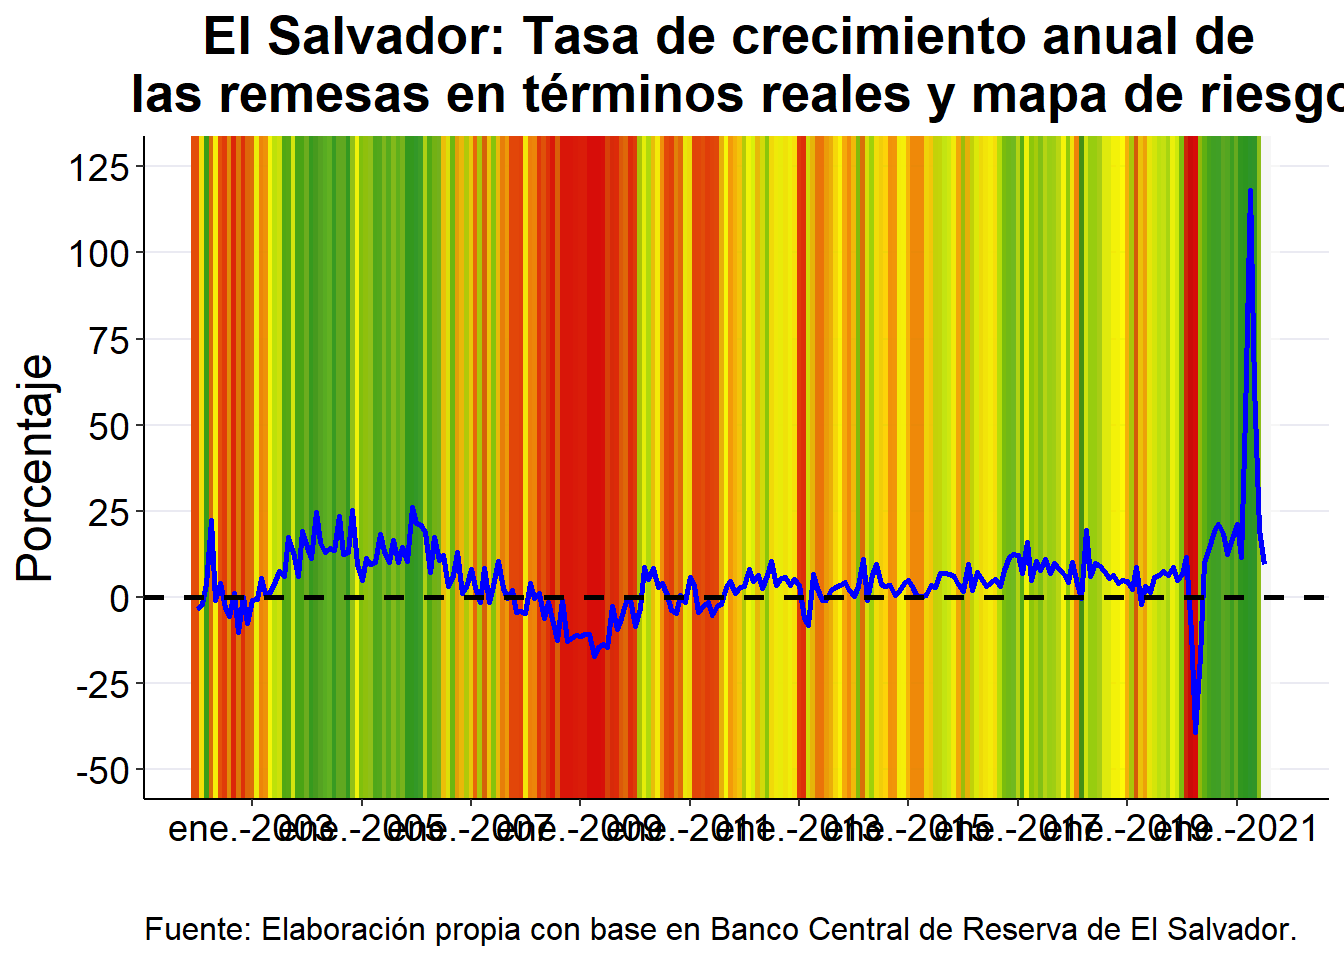
\includegraphics{index_files/figure-latex/unnamed-chunk-2-1.pdf}

  \bibliography{book.bib,packages.bib}

\end{document}
